\paragraph{Sơ đồ tuần tự luồng Pha local handler gửi email xác nhận thanh toán VIP}

Luồng nghiệp vụ này mô tả
\texttt{SubscriptionPurchasedEventHandler} trong Payment Service xử lý domain event nội bộ sau khi thanh toán thành công. Handler lấy email từ metadata của transaction, lấy tên người dùng từ Supabase Profile Service, lấy tên gói từ Payment DB và gọi Brevo Email Adapter để gửi email xác nhận.

\begin{figure}[H]
\centering
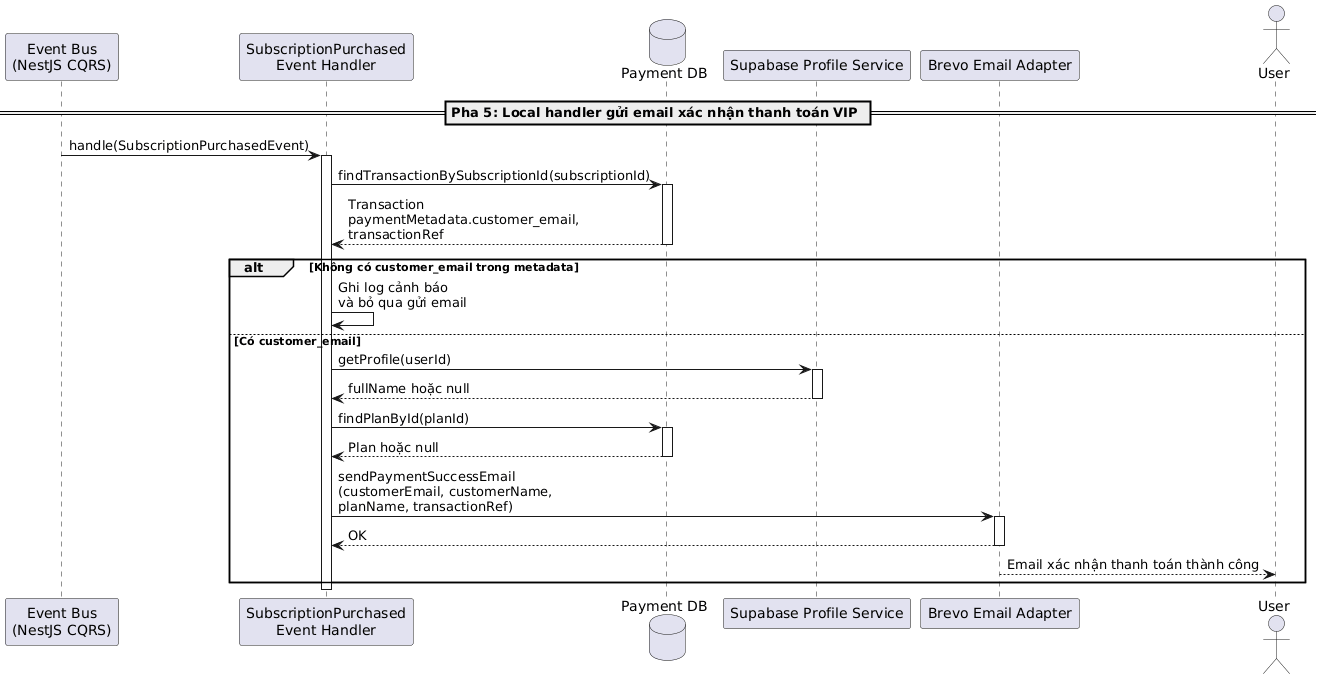
\includegraphics[scale = 0.2]{contents/Sequence/UML-Sequence-PaymentSendVipConfirmationEmail.png}
\caption{Sơ đồ tuần tự luồng Pha local handler gửi email xác nhận thanh toán VIP}
\end{figure}

\subparagraph{Các thành phần tham gia}

\begin{table}[H]
\centering
\renewcommand{\arraystretch}{1.3}

\begin{tabular}{|l|l|p{5cm}|}
\hline
\textbf{Thành phần} & \textbf{Phân loại} & \textbf{Vai trò trong hệ thống} \\ \hline
Event Bus (NestJS CQRS) & Component & Phát sự kiện thanh toán cho local event handler. \\ \hline
SubscriptionPurchased Event Handler & Component & Lấy dữ liệu cần thiết và điều phối gửi email xác nhận thanh toán. \\ \hline
Payment DB & Database & Cung cấp transaction metadata, transaction reference và thông tin plan. \\ \hline
Supabase Profile Service & External Service & Cung cấp \texttt{fullName} của người dùng; email gửi thông báo được lấy từ transaction metadata. \\ \hline
Brevo Email Adapter & External Service & Gửi email xác nhận thanh toán thành công. \\ \hline
User & Actor & Nhận email xác nhận giao dịch VIP. \\ \hline
\end{tabular}
\caption{Các thành phần tham gia luồng pha local handler gửi email xác nhận thanh toán VIP}
\end{table}

\subparagraph{Mô tả tổng quan}

\begin{itemize}
\item \textbf{Nhận thông điệp sự kiện:}
Bộ xử lý sự kiện nhận thông điệp sự kiện mua gói thuê bao VIP thành công từ hệ thống truyền tin nội bộ.
\item \textbf{Lấy thông tin liên hệ:}
Bộ xử lý tìm thông tin giao dịch để lấy email khách hàng và mã tham chiếu thanh toán. Nếu không tìm thấy thông tin email, bộ xử lý ghi lại cảnh báo và bỏ qua việc gửi thư điện tử.
\item \textbf{Lấy thông tin bổ sung:}
Bộ xử lý gọi dịch vụ thông tin cá nhân để lấy họ tên đầy đủ của người dùng (sử dụng tên mặc định nếu không có) và lấy thông tin chi tiết của gói dịch vụ đã mua.
\item \textbf{Gửi thư điện tử:}
Bộ xử lý gửi yêu cầu qua dịch vụ gửi thư điện tử bên ngoài để gửi thư xác nhận thanh toán thành công và kích hoạt gói thuê bao VIP cho người dùng.
\end{itemize}
